For this project, we defined our specifications to ensure a properly structured
project, with defined goals and constraints.

This include :

\begin{itemize}
    \item Mechanical constraints :
          \begin{itemize}[noitemsep]
              \item Rocket shall be at least 1m tall (personal preference).
              \item Rocket should have a thin profile compared to the height
                    (\ref{chap:controller}).
              \item Rocket should have a CG/CL (center of gravity over center of lift, which
                    determines stability).
              \item Model shall be stabilized upright and controlled by control surfaces, placed at
                    the top of the rocket.
              \item The rocket shall be recoverable using a parachute to land smoothly.
          \end{itemize}

    \item Electronic constraints :
          \begin{itemize}[noitemsep]
              \item Acquisition of the acceleration, position, pression and speed.
              \item Local treatement by an microcontroller on board.
              \item Backup of measured data for cold analysis.
              \item The system shall be powered from batteries.
              \item The rocket shall be easily localizable using a buzzer, a bright LED or a
                    Wireless protocol.
          \end{itemize}

    \item   The system shall handle the maximal acceleration of the system, around 15g.
    \item   The system shall handle speeds up to $150 \si{\meter\per\second}$.
\end{itemize}

\vspace{0.8 cm}

All of these specifications leads to this first approximation of the rocket
schematic :

\begin{figure}[!hbt]
    \centering
    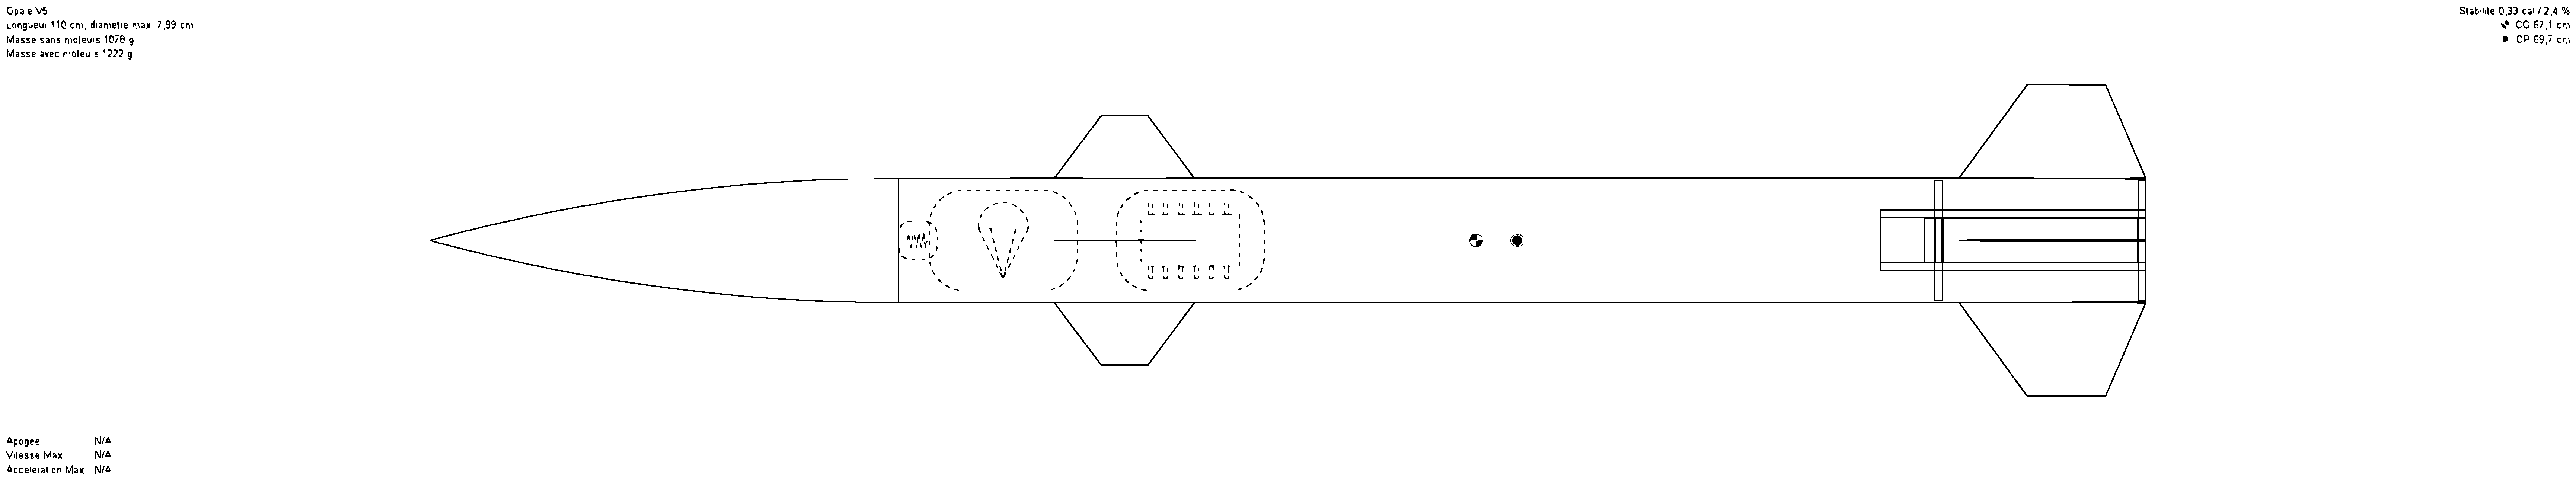
\includegraphics[width=\SchematicWidth]{\Images/mechanical/RocketSchematics.eps}
    \caption{First schematic}
\end{figure}
\FloatBarrier

